\documentclass[letterpaper, 12pt]{article}

\usepackage{amsmath}
\usepackage{graphicx}
\usepackage{{subfig}}
\linespread{1.3}
\begin{document}


\title{6.036 Project 2 \vspace{8mm}}
\author{ Dimitris Koutentakis}
\date{11 April 2017}
\maketitle
For this project I used the following:
\begin{itemize}
    \item Python 3.6.0
    \item Numpy 1.12.1
    \item Scipy 0.19.0
    \item PyYAML 3.12
    \item Cython 0.25.2
    \item h5py 2.7.0
    \item theano 0.9.0
    \item keras 2.0.2
    \clearpage
\end{itemize}
\section*{Problem 1}
All implemented code is attached.
\begin{enumerate}
\item[4.]
The final error after running main.py, is:
\begin{align*}
    \epsilon = 0.1005
\end{align*}
    \item[5.] The temperature parameter $\tau$ affects the magnitude of the $\theta$ vector we get. In specific, a larger $\tau$ would lead to a smaller updates, and thus to a $\theta$ that is smaler than otherwise. A larger value of $\tau$ would have a larger probability of a smaller $\theta$ and the opposite.
    \item[6.]  Changing the teperature parameter gives the following results:
    \begin{itemize} 
        \item For $\tau = 0.5$, we have an error of $0.084$.
        \item For $\tau = 1$, we get an error of $ 0.1005$.
        \item For $\tau = 2$, we get an error of  $0.1261$.
    \end{itemize}
    It seems that the larger the temperature factor, the larger the error rate. This suggests that the 
    probability distribution is normal and the magnitude change with the value of $\tau$
    \item[9.] When classifying the points by their $(mod3)$ labels, the error drops by a considerable amount.
    The new error we get is \begin {align*}     \epsilon=0.0768     \end{align*}
    If on the other hand we also train the samples on the $(mod3)$ values, then the error jumps up to a value of: 
    \begin{align*}\epsilon=0.1872 \end{align*}
    It is pretty obvious why the error changes so much by applying $(mod3)$ at different places. For example when training the points in the full space, but only checking their labels in the 3 dimensional space, it means that some of that error gets lost. Any points with label $Y=1$ that were mis-classified as a 4 or a 7, will end up counting as "correct", as the $(mod3)$ value of all these points is the same.\\
    On the other hand, when we train the points on 3 values, then each misclassification ends up counting for more. 
\end{enumerate}
\vspace{3mm}
\section*{Problem 2}
All code for Problem 2 is attached.

\begin{enumerate}
    \item[3.] By implementing the PCA feature, and recalculating the error of the regression with the PCA data, we get an error that is very close to the original error. In specific, we now get an error of:
    \begin{align*}\epsilon = 0.1483 \end{align*}
    \item The original and reconstructed pictures can be viewed below:
        \begin{figure}[!ht]
        \centering
        \subfloat[Original picture]{
\includegraphics[width=0.5\textwidth]{2_5_b.png}\label{fig:f1}}
        \hfill
        \subfloat[Recunstructed picture]{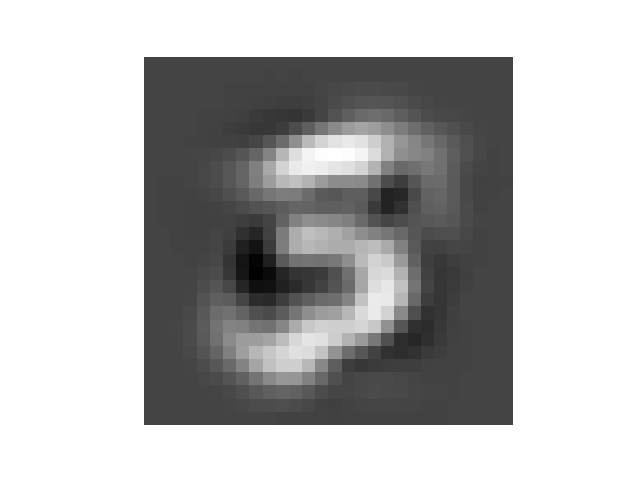
\includegraphics[width=0.5\textwidth]{2_5_a.png}\label{fig:f2}}
        \caption{First reconstruction}
        \end{figure}
        \begin{figure}[!ht]
        \centering
        \subfloat[Original picture]{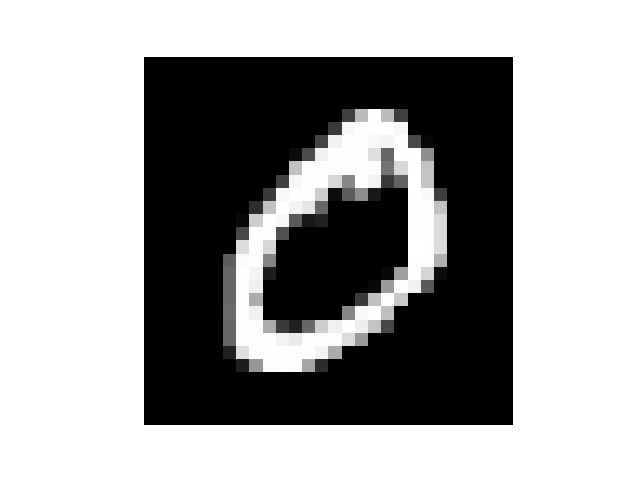
\includegraphics[width=0.5\textwidth]{2_5_d.png}\label{fig:f3}}
        \hfill
        \subfloat[Recunstructed picture]{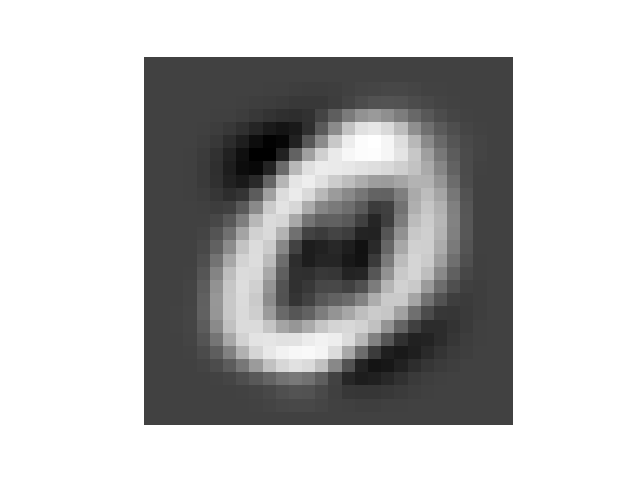
\includegraphics[width=0.5\textwidth]{2_5_c.png}\label{fig:f4}}
        \caption{Second reconstruction}
        \end{figure}

\clearpage

     
    \item[6.] The cubic feature mapping $\Phi(x)$, is the following:
    \begin{align*}
        \Phi(x)=[x_1^3, \sqrt3x_1^2x_2, \sqrt3x_1^2, \sqrt3x_1x_2^2, \sqrt6x_1x_2, \sqrt3x_1, x_2^3, \sqrt3x_2^2, \sqrt3x_2, 1]
    \end{align*}
    \item[7.] After implementing the cubic feature Kernel, we get an error much lower than any other method so far. The cubic feature kernel error is:
    \begin{align*}
        \epsilon=0.0865
    \end{align*}
 
\end{enumerate}
\vspace{3mm}
\section* {Problem 3}
All code for problem 3 is attached.
\begin{enumerate} 
    \item[4.] In order to improve the efficiency of the training and accuracy of our network, we have to update the learning rate. This can be done in at least two ways.
    \begin{itemize}
        \item Decrease the learning rate $\eta$ as the number of updates increases,
        \item Decrease the learning rate $\eta$ when the magnitude of the gradient decreases.
    \end{itemize} 
    \item [5.] The danger of having too many hidden units in your network is twofold.
    \begin{itemize}
        \item First, computation cost increases significantly and
        \item Secondly there is a large risk of overfitting to our data.
    \end{itemize}
    \item [6.] If we run the code for a significantly larger number of epochs, the training accuracy will keep getting better. The more the epochs, the better the training accuracy. \\
    On the other hand, as we increase the number of epochs, the test accuracy will initially increase and at some point will start declining, as we will be overfitting our data.
    \item[7.] In order to hit the sweetspot where we train the network well, but do not overfit our data, we will have to try several different values of epochs and pick the one that does not overfit, while presenting the best performance.
\end{enumerate}
\vspace{3mm}
\section*{Problem 4}
The code for Problem 4 is attached.
\begin{enumerate}
    \item The initial accuracy we get after the first training, is:
    \begin{align*}
        \text{Accuracy on test set: } 0.9168
    \end{align*}
    \item I tried several things in order to increase the accuracy, however it seemed like just tweaking the learning rate and the momentum factors was enough to increase the accuracy to above 98\%.
    The changes I made were:
    \begin{itemize}
    \item Increase learning rate to \verb|lr=0.1|
    \item Change momentum factor to: \verb|momentum = 0.65| 
    \end{itemize}
    These changes ended up giving me an accuracy of:
    \begin{align*}
        \text{Accuracy on test set: } 0.9806
    \end{align*}
    \item After implementing all of the layers for the model, we getting the following accuracies:
    \begin{align*}
        \text{Test data accuracy: } 0.9333
    \end{align*}
    \begin{align*}
        \text{Training data accuracy: } 0.9847
    \end{align*}
    
\end{enumerate}
\vspace{3mm}
\section*{Problem 5}

\begin{enumerate}
\item  The model.compile line activates our network model and configures the learning process with the parameters we pass. In specific, it has the 'categorical\_crossentropy' loss function, uses stochastic gradient descent to optimize the model and accurazy in order to gauge how good it performs.  \\
    The model.fit line does the approximation and the training of the model. In our case, it uses the training images as well as the two labels (for the two images). It runs for 30 epochs and has a batch size of 64.
        \item For the observation section, I was able to increase the accuracy quite a bit.
        \begin{itemize}
            
        
        \item Initially, mlp.py returned: \\ \verb|'dense\_2\_acc': 0.90400000000000003, 'dense\_3\_acc': 0.89324999999999999|
        \item  For the first model, I added a layer of 100 neurons to mlp.py. The new accuracies were: \\ \verb| 'dense_3_acc': 0.91100000000000003, 'dense_4_acc': 0.90200000000000002|. The time did not change much.
        \item For the second architecture I added two layers of 1000 neurons each, which resulted in: \\ \verb|'dense_4_acc': 0.91900000000000004, 'dense_5_acc': 0.90275000000000005| and a slightly longer runtime.
        \item for my last test, I added a convolution, a pooling and a flattening layer, and reduced the number of epochs to 16. This resulted in the largest increase in acuracy increase, giving: \\ \verb| dense_2_acc: 0.9633 - dense_3_acc: 0.9534 |. This method however took much longer to run (more than 10 times longer than the other methods).
        \end{itemize}
        In the end, I believe that my second attempt had the best result for the runtime.

\end{enumerate}


\end{document}